\subsection{Description of the algorithm}
First proposed in \cite{aschenbrenner2007finite} and formalized in \cite{Brouwer09e}, the classical Buchberger's algorithm~\cite{buchberger1965algorithmus} may be adapted to the equivariant setting in a straightforward way.

Let $R = K\mon$ with $\Pi$ acting on $\mon$, and let $\leq$ be a $\Pi$-respecting monomial order.  For $f,g \in R$, we say that $g$ {\em $\Pi$-reduces} $f$ if $\LT g |_{\Pi} \LT f$ and the reduction is $f - \frac{\LC(f)}{\LC(g)}mg$ where $m \in \mon *\Pi$ is such that $\LT f = m\LT g$ (and $\LC(f)$ denotes the lead coefficient of $f$).  For $G \subseteq R$, a {\em $\Pi$-normal form} of $f$ with respect to $G$, denoted $\NF_{\Pi G}(f)$, is the result of repeated $\Pi$-reductions of $f$ by elements of $G$ until no more reductions are possible.  Equivalently, $\NF_{\Pi G}(f)$ is a normal form of $f$ with respect to $\Pi G$.

The equivariant Buchberger's algorithm is described below, which departs from the conventional Buchberger's algorithm only at the step of adding new S-pairs to the list $S$.  The necessity and extent of this departure becomes clear with the definition of $O_{f,g}$ and the {\em finite S-pair condition} (Definition~\ref{def:finite-s-pair}) that are given after the description of the algorithm.

\begin{algorithm}[Brouwer--Draisma \cite{Brouwer09e}]\label{alg:Buchberger}
$G = \alg{Buchberger}(F)$
\begin{algorithmic}[1]
\REQUIRE $F$ is a finite set of elements in $R = K\mon$ with $\Pi$ acting on $\mon$ and satisfying the finite S-pair condition.
\ENSURE $G$ is $\Pi$-equivariant Gr\"obner basis of $\ideal{F}_{\Pi}$.

\smallskip \hrule \smallskip

\STATE $G\gets F$
\STATE $S\gets \bigcup_{f,g\in G} O_{f,g}$
\WHILE{$S\neq\emptyset$}
	\STATE pick $(h_1,h_2) \in S$
	\STATE $S\gets S\setminus\{(h_1,h_2)\}$ 
	\STATE $h \gets \NF_{\Pi G}(h_1 - \frac{\LC(h_1)}{\LC(h_2)}h_2)$
  	\IF{$h \neq 0$}
		\STATE $G\gets G\cup \{h\}$
		\STATE $S\gets S\cup \left(\bigcup_{g\in G}O_{g,h}\right)$
	\ENDIF
\ENDWHILE
\smallskip \hrule \smallskip
\end{algorithmic}
\end{algorithm}

Given $f,g \in R$ define:
 \[ \C S_{f,g} := \{(m_1f,m_2g) \mid m_1,m_2 \in \mon * \Pi \text{ such that } \LT m_1f = \LT m_2g\}. \]
This set is closed under the diagonal action of $\mon *\Pi$, making $\C S_{f,g}$ a $\mon *\Pi$-module.  

\begin{definition}\label{def:buchberger-criterion}
A set $G \subseteq R$ satisfies the {\em equivariant Buchberger criterion} if for all $(h_1,h_2) \in \bigcup_{f,g\in G} \C S_{f,g}$:
 \[ \NF_{\Pi G}(h_1 - \tfrac{\LC(h_1)}{\LC(h_2)}h_2) = 0. \]
\end{definition}

The set $G$ is a $\Pi$-equivariant Gr\"obner basis of $\ideal{G}_{\Pi}$ if and only if it satisfies the equivariant Buchberger criterion.  The proof of this fact follows by applying the usual Buchberger criterion to the set $\Pi G$ (see Theorem 2.5 of \cite{Brouwer09e}).

For each pair $f,g \in G$, we need not check the criterion on every pair in the infinite set $\C S_{f,g}$.  It is instead sufficient to check on a $\mon * \Pi$ generating set of $\C S_{f,g}$, which we denote $O_{f,g}$.  Still, in general, it may be that no finite generating set of $\C S_{f,g}$ exists, in which case we cannot apply the algorithm in finite time.

\begin{definition}\label{def:finite-s-pair}
 A $\Pi$-algebra $R = K\mon$ has the {\em finite S-pair condition} if for any $f,g \in R$, the set $\C S_{f,g}$ is finitely generated as a $\mon * \Pi$-module.  In \cite{Brouwer09e}, this condition is referred to as ``EGB4.''
\end{definition}

When $\Pi$ is trivial and $R$ is a polynomial ring (the setting of the conventional Buchberger's algorithm), $\C S_{f,g}$ is generated by a single pair $(m_1 f,\; m_2 g)$ where:
$$
m_1 = \lcm(\LT f, \LT g)/\LT(f),\quad
m_2 = \lcm(\LT f, \LT g)/\LT(g)
\,.
$$  
This generator is typically referred to as the {\em S-pair} of $f,g$.  Therefore, $R$ in this case satisfies the finite S-pair condition, and the equivariant Buchberger's algorithm specializes to the conventional Buchberger's algorithm.

\begin{proposition}
 If $R$ is a polynomial ring $R = K[Y]$ with $\Inc$-action on $[Y]$ satisfying the finite width condition, then $R$ has the finite S-pair condition.
\end{proposition}
\begin{proof}
 Fix $f,g \in R$.
 Since $R$ is a polynomial ring, for fixed $\sigma_1,\sigma_2 \in \Inc$, all elements of $\C S_{f,g}$ of the form $(m_1\sigma_1 f, m_2\sigma_2 g)$ with $m_1,m_2 \in \mon$ are monomial multiplies of the usual S-pair of $\sigma_1 f, \sigma_2 g$:
  \[ \left(\frac{m}{\LT \sigma_1 f} \sigma_1 f,\; \frac{m}{\LT \sigma_2 g} \sigma_2 g\right),\]
 where $m = \lcm(\LT \sigma_1 f,\LT \sigma_2 g)$.

 Any $f,g \in R$ have finite width so $\sigma_1 f$ depends only on $\sigma_1|_{[w(f)]}$, and similarly for $\sigma_2 g$.  In fact, we can always factor the pair as:
  \[ (\sigma_1 f, \sigma_2 g) = \rho(\sigma'_1 f, \sigma'_2 g),\]
 for some $\rho \in \Inc$, while $\sigma'_1:[w(f)] \to [w(f) + w(g)]$ and $\sigma'_2:[w(g)] \to [w(f) + w(g)]$ are strictly increasing functions.  Here $\sigma'_1$ and $\sigma'_2$ are chosen to ``interlace'' the variables of $f$ and $g$ in the same way as $\sigma_1,\sigma_2$.  (To consider $\sigma'_1,\sigma'_2$ as elements of $\Inc$, take any choice of extensions to maps on $\B N$.)
 
 Then, $\C S_{f,g}$ is generated by the finite set of pairs of the form:
  \[ \left(\frac{m}{\LT \sigma'_1 f} \sigma'_1 f,\; \frac{m}{\LT \sigma'_2 g} \sigma'_2 g\right),\]
 with $\sigma'_1:[w(f)] \to [w(f) + w(g)]$ and $\sigma'_2:[w(g)] \to [w(f) + w(g)]$ where $m = \lcm(\LT \sigma'_1 f,\LT \sigma'_2 g)$.
\end{proof}
\begin{figure}[ht]\label{fig:interlace}
  \centering
  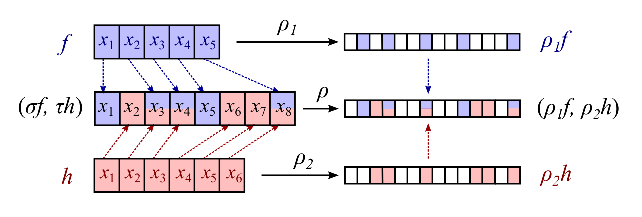
\includegraphics[width=.9\columnwidth]{incmap.pdf}
  \caption{For $f$ and $g$ of width 5 and 6 respectively, any S-pair, $(\rho_1 f,\rho_2 g)$, is in the orbit of some S-pair obtained from an ``interlacing'' of $[5]$ and $[6]$, $(\sigma f,\tau g)$.}
\end{figure}

We note that Algorithm \ref{alg:Buchberger} is guaranteed to terminate when $R$ is $\Pi$-Noetherian.  Let $G_0,G_1,\ldots$ be the value of $G$ at each step.  The initial ideals of these sets form a strictly increasing chain of $\Pi$-invariant monomial ideals:
 \[ \ideal{\LT G_0}_\Pi \subsetneq \ideal{\LT G_1}_\Pi \subsetneq \cdots,\]
which must terminate.  However, without Noetherianity, we offer no termination guarantee of the algorithm as stated above, even when a finite equivariant Gr\"obner basis for the ideal exists.  Algorithm~\ref{alg:truncBuch} is a modification of the algorithm which repairs this when $\Pi = \Inc$, a finite equivariant Gr\"obner basis exists, and the truncated rings $R_n$ are Noetherian.

\subsection{Termination of $\Inc$-equivariant Buchberger}
Let $R = K\mon$ with $\Inc$ action on $\mon$, with $R$ satisfying the finite width and finite S-pair conditions, and with each truncation $R_n$ a Noetherian ring.  Let $I \subseteq R$ be a $\Inc$-invariant ideal which is $\Inc$-generated by finite set $F$, and, moreover, has finite $\Inc$-equivariant Gr\"obner basis $G$.  Define the {\em generator truncation} of $I$ to be $\tilde{I}_{F,n} := \ideal{\Inc F \cap R_n} \cap R_n$.  Note that $\tilde{I}_{F,n} \subseteq I_n$, but, in general, equality does not hold.  For $f \in I$, define $w_F(f)$ to be the minimum value of $n$ for which $f \in \tilde{I}_{F,n}$.

The truncated EGB algorithm takes a finite generating set $F$ as its input.  For each successive $n \geq w(F)$, it computes a set $G_n$ such that $\Inc G_n \cap R_n$ is a Gr\"obner basis for $\tilde{I}_{F,n}$.  Then it checks if $G_n$ is a $\Inc$-equivariant Gr\"obner basis of $I$ using the equivariant Buchberger criterion (Definition~\ref{def:buchberger-criterion}), and if so returns $G_n$.

\begin{algorithm}\label{alg:truncBuch}
$G = \alg{TruncatedEGB}(F)$
\begin{algorithmic}[1]
\REQUIRE $F$ is a finite set of elements in $R = K\mon$ with $\Inc$ acting on $\mon$, $R$ satisfies the finite width and finite S-pair conditions, and each $R_n$ is Noetherian.
\ENSURE $G$ is a $\Inc$-equivariant Gr\"obner basis of $I := \ideal{F}_{\Inc}$.

\smallskip \hrule \smallskip

\STATE $G\gets F$
\STATE $n\gets w(F)$
\WHILE{$G$ not a $\Inc$-equivariant Gr\"obner basis of $I$}
	\STATE $G\gets$ Gr\"obner basis of $\tilde{I}_{F,n}$
	\STATE $n \gets n+1$
\ENDWHILE
\smallskip \hrule \smallskip
\end{algorithmic}
\end{algorithm}

\begin{proof}[Proof of termination (supposing a finite EGB for $I$)]
For each $n$, let $G_n$ denote the value of $G$ after that step.  Computing $G_n$ is a finite process since it takes place in $R_n$, which is Noetherian.  $G_n$ is a finite set, and so it has a finite number of S-pairs to be checked.  Therefore, testing whether $G_n$ is a $\Inc$-equivariant Gr\"obner basis is finite.

It remains to be proved that $G_n$ is a $\Inc$-equivariant Gr\"obner basis for some value of $n$.  If $H$ is a $\Inc$-equivariant Gr\"obner basis of $I$, for any $h \in H$ we have $h \in \tilde{I}_{F,n}$ for all $n \geq w_F(h)$, so $\LT(h) \in \LT(\tilde{I}_{F,n})$.  Thus, there is some $g \in G_n$ with $\LT(g)|_{\Inc} \LT(h)$.  For $n = \max_{h\in H} w_F(h)$, the initial ideal $\ideal{\LT(G_n)}_{\Inc}$ then necessarily contains $\ideal{\LT(H)}_{\Inc}$, and so $G_n$ is a $\Inc$-equivariant Gr\"obner basis of $I$.
\end{proof}

In practice, $G_n$ can be computed either using a traditional Gr\"obner basis algorithm on input $\Inc F \cap R_n$ or using an equivariant Buchberger's algorithm on input $F$ with the following two caveats:
\begin{itemize}
 \item Consider only S-pairs $(m_1f, m_2g)$ with $m_1f$ and $m_2g$ both having width $\leq n$,
 \item Perform only reductions such that the outcome has width $\leq n$.
\end{itemize}
Moreover, we do not need to restart the algorithm from scratch for each $n$: $G_{n-1} \cup F$ can be used as the input for the $n$th step instead of $F$.

Suppose $R$ has the form $K[Y]$ and each $R_n = K[Y_n]$ for some $Y_n \subseteq Y$.  If $\leq$ is a width order (a monomial order such that $w(a) < w(b)$ implies $a < b$), the second condition is satisfied automatically since reductions cannot increase the width.  Therefore, the normal form of a given S-pair does not depend on $n$ and only needs to be computed once.  As a result, we can use Algorithm \ref{alg:Buchberger}, queuing S-pairs by width so that the smallest width S-pairs are considered first.  The algorithm terminates once the queue is empty.  A separate check for whether $G_n$ is a $\Inc$-equivariant Gr\"obner basis for $I$ is not needed since this is equivalent to reducing all S-pairs in the queue.

\subsection{Macaulay2 package}

We have implemented several strategies for computing equivariant Gr\"obner bases in a package: \begin{center}
\verb|EquivariantGB|~(see {\tt http://rckr.one/EquivariantGB.html}) 
\end{center}
for Macaulay2~\cite{grayson2002macaulay}, a software system for computational algebraic geometry and commutative algebra.

The main command of our Macaulay2 package, \verb|egb|, has an optional argument that determines how the computation is done:
\begin{itemize}
\item 
\verb|egb(...,Algorithm=>Buchberger)| uses Algorithm~\ref{alg:Buchberger},
\item 
\verb|egb(...,Algorithm=>Incremental)| uses Algorithm~\ref{alg:truncBuch},
\item 
\verb|egb(...,Algorithm=>Signature)| uses the approach in~\S\ref{sec:signature}.
\end{itemize}

\begin{remark}\label{rem:4ti2}
With the assumptions of Theorem~\ref{thm:DEKL}, one can operate  with truncated toric ideals and use specialized lattice based Gr\"obner bases algorithms to improve performance. 
Our Macaulay2 command for that, \verb|egbToric|, outsources heavy computation to \verb|4ti2|~(see \cite{4ti2}),  a special software package for algebraic, geometric, and combinatorial problems on linear spaces.   
\end{remark}
